\documentclass[conference]{IEEEtran}
\usepackage{cite}
\usepackage{amsmath,amssymb,amsfonts}
\usepackage{graphicx}
\usepackage{textcomp}
\usepackage{xcolor}
\usepackage{booktabs}
\usepackage{multirow}
\usepackage{hyperref}
\usepackage{algorithm}
\usepackage{algorithmic}
\usepackage{subcaption}
\usepackage{float}

\def\BibTeX{{\rm B\kern-.05em{\sc i\kern-.025em b}\kern-.08em
    T\kern-.1667em\lower.7ex\hbox{E}\kern-.125emX}}

\begin{document}

\title{DeepVIO: Deep Visual-Inertial Odometry with FiLM Fusion on Synthetic Data}

\author{\IEEEauthorblockN{Aditya Patwardhan, Bradley}
\IEEEauthorblockA{Worcester Polytechnic Institute\\
RBE 549 --- Computer Vision, Spring 2026\\
}}

\maketitle

\begin{abstract}
We present DeepVIO, a deep learning approach to visual-inertial odometry (VIO) that fuses monocular camera images with inertial measurement unit (IMU) data for 6-DoF relative pose estimation. We develop a complete synthetic data generation pipeline using Blender and implement three model variants---vision-only (DeepVO), IMU-only (DeepIO), and fused (DeepVIO). Our initial experiments revealed a critical data quality bottleneck: 54\% of training images were too featureless for visual odometry. After systematic diagnosis and dataset curation, we introduce two key architectural improvements: (1) a pretrained ResNet-18 visual encoder replacing a from-scratch CNN, and (2) Feature-wise Linear Modulation (FiLM) for sensor fusion with a two-stage training strategy that solves the modality imbalance problem. Our best model achieves a 92\% reduction in test loss (0.3017 $\to$ 0.0237) and 1.5m average Absolute Trajectory Error on test sequences, with the fused model outperforming vision-only for the first time.
\end{abstract}

\begin{IEEEkeywords}
Visual-Inertial Odometry, Deep Learning, Sensor Fusion, FiLM Conditioning, Synthetic Data
\end{IEEEkeywords}

% ======================================================================
\section{Introduction}
% ======================================================================

Visual-Inertial Odometry (VIO) estimates the 6-DoF pose of a moving platform by fusing visual features from cameras with inertial measurements from accelerometers and gyroscopes. Classical approaches such as MSCKF~\cite{mourikis2007} and VINS-Mono~\cite{qin2018} achieve high accuracy through tightly-coupled filtering or optimization, but rely on hand-crafted feature pipelines that require careful tuning.

Recent learning-based approaches have demonstrated promising results. DeepVO~\cite{wang2017} showed that a CNN-LSTM architecture with pretrained FlowNet features can learn visual odometry end-to-end. VINet~\cite{clark2017} extended this to incorporate IMU data through concatenation-based fusion. However, these approaches face several challenges: (1) the need for large, diverse training data with accurate ground truth, (2) the \textit{modality imbalance problem} where the faster-converging modality suppresses the other during joint training~\cite{wang2020multimodal}, and (3) poor generalization to unseen environments.

In this work, we make the following contributions:
\begin{itemize}
    \item A synthetic data generation pipeline using Blender producing synchronized camera-IMU sequences with perfect ground truth.
    \item Systematic diagnosis of data quality as the primary bottleneck, with quantitative image quality analysis.
    \item Feature-wise Linear Modulation (FiLM)~\cite{perez2018} for visual-inertial fusion, replacing naive concatenation.
    \item A two-stage training strategy that solves the modality imbalance problem by pretraining the visual encoder before joint fusion training.
\end{itemize}

% ======================================================================
\section{Related Work}
% ======================================================================

\subsection{Classical Visual-Inertial Odometry}
MSCKF~\cite{mourikis2007} introduced tightly-coupled VIO using an Extended Kalman Filter with a sliding window of camera poses. VINS-Mono~\cite{qin2018} extended this with nonlinear optimization and loop closure. ORB-SLAM~\cite{mur2015} demonstrated robust visual SLAM using ORB features. These methods achieve high accuracy but require engineered feature pipelines.

\subsection{Learned Visual Odometry}
DeepVO~\cite{wang2017} pioneered end-to-end visual odometry using a FlowNet-S~\cite{dosovitskiy2015} CNN encoder pretrained on synthetic optical flow, followed by a two-layer LSTM. The key finding was that pretrained visual features dramatically improve performance. TartanVO~\cite{wang2021} demonstrated strong generalization by training on the TartanAir~\cite{wang2020tartanair} synthetic dataset with PWC-Net~\cite{sun2018} optical flow as input.

\subsection{Learned Visual-Inertial Fusion}
VINet~\cite{clark2017} first combined learned visual features with IMU data using concatenation. DeepVIO~\cite{han2019} improved upon this by using explicit optical flow features and separate LSTM branches. SelectFusion~\cite{chen2019} introduced soft attention gating that learns when to trust each modality. The modality imbalance problem---where one sensor dominates gradient flow during joint training---has been identified as a key challenge in multi-modal learning~\cite{wang2020multimodal}.

\subsection{Feature-wise Linear Modulation}
FiLM~\cite{perez2018} was introduced for visual reasoning, where a conditioning signal generates per-channel scale ($\gamma$) and shift ($\beta$) parameters that modulate feature maps: $\text{FiLM}(\mathbf{x} | \gamma, \beta) = \gamma \odot \mathbf{x} + \beta$. This provides a richer interaction than concatenation, allowing one modality to amplify or suppress specific feature channels of another.

% ======================================================================
\section{Methodology}
% ======================================================================

\subsection{Data Generation Pipeline}

We develop a synthetic data generation pipeline using Blender 4.5 with the EEVEE rendering engine (Fig.~\ref{fig:data_pipeline}).

\textbf{Scene Setup.} A 200m $\times$ 200m ground plane is textured with tiled photographic or procedural textures. Twenty randomly placed 3D primitives (cubes, cylinders, cones of 0.5--4m scale) provide depth variation and parallax cues. The camera is positioned at 10--15m altitude with a 20mm lens (84$^\circ$ horizontal FOV).

\textbf{Trajectory Generation.} Four trajectory families---figure-8, spiral, Lissajous, and linear---with smooth 6-DoF motion over 20 seconds. Camera poses are sampled at 10~Hz (200 frames/sequence). Figure~\ref{fig:traj_types} illustrates the four trajectory families used in our data generation pipeline.

\begin{figure}[t]
    \centering
    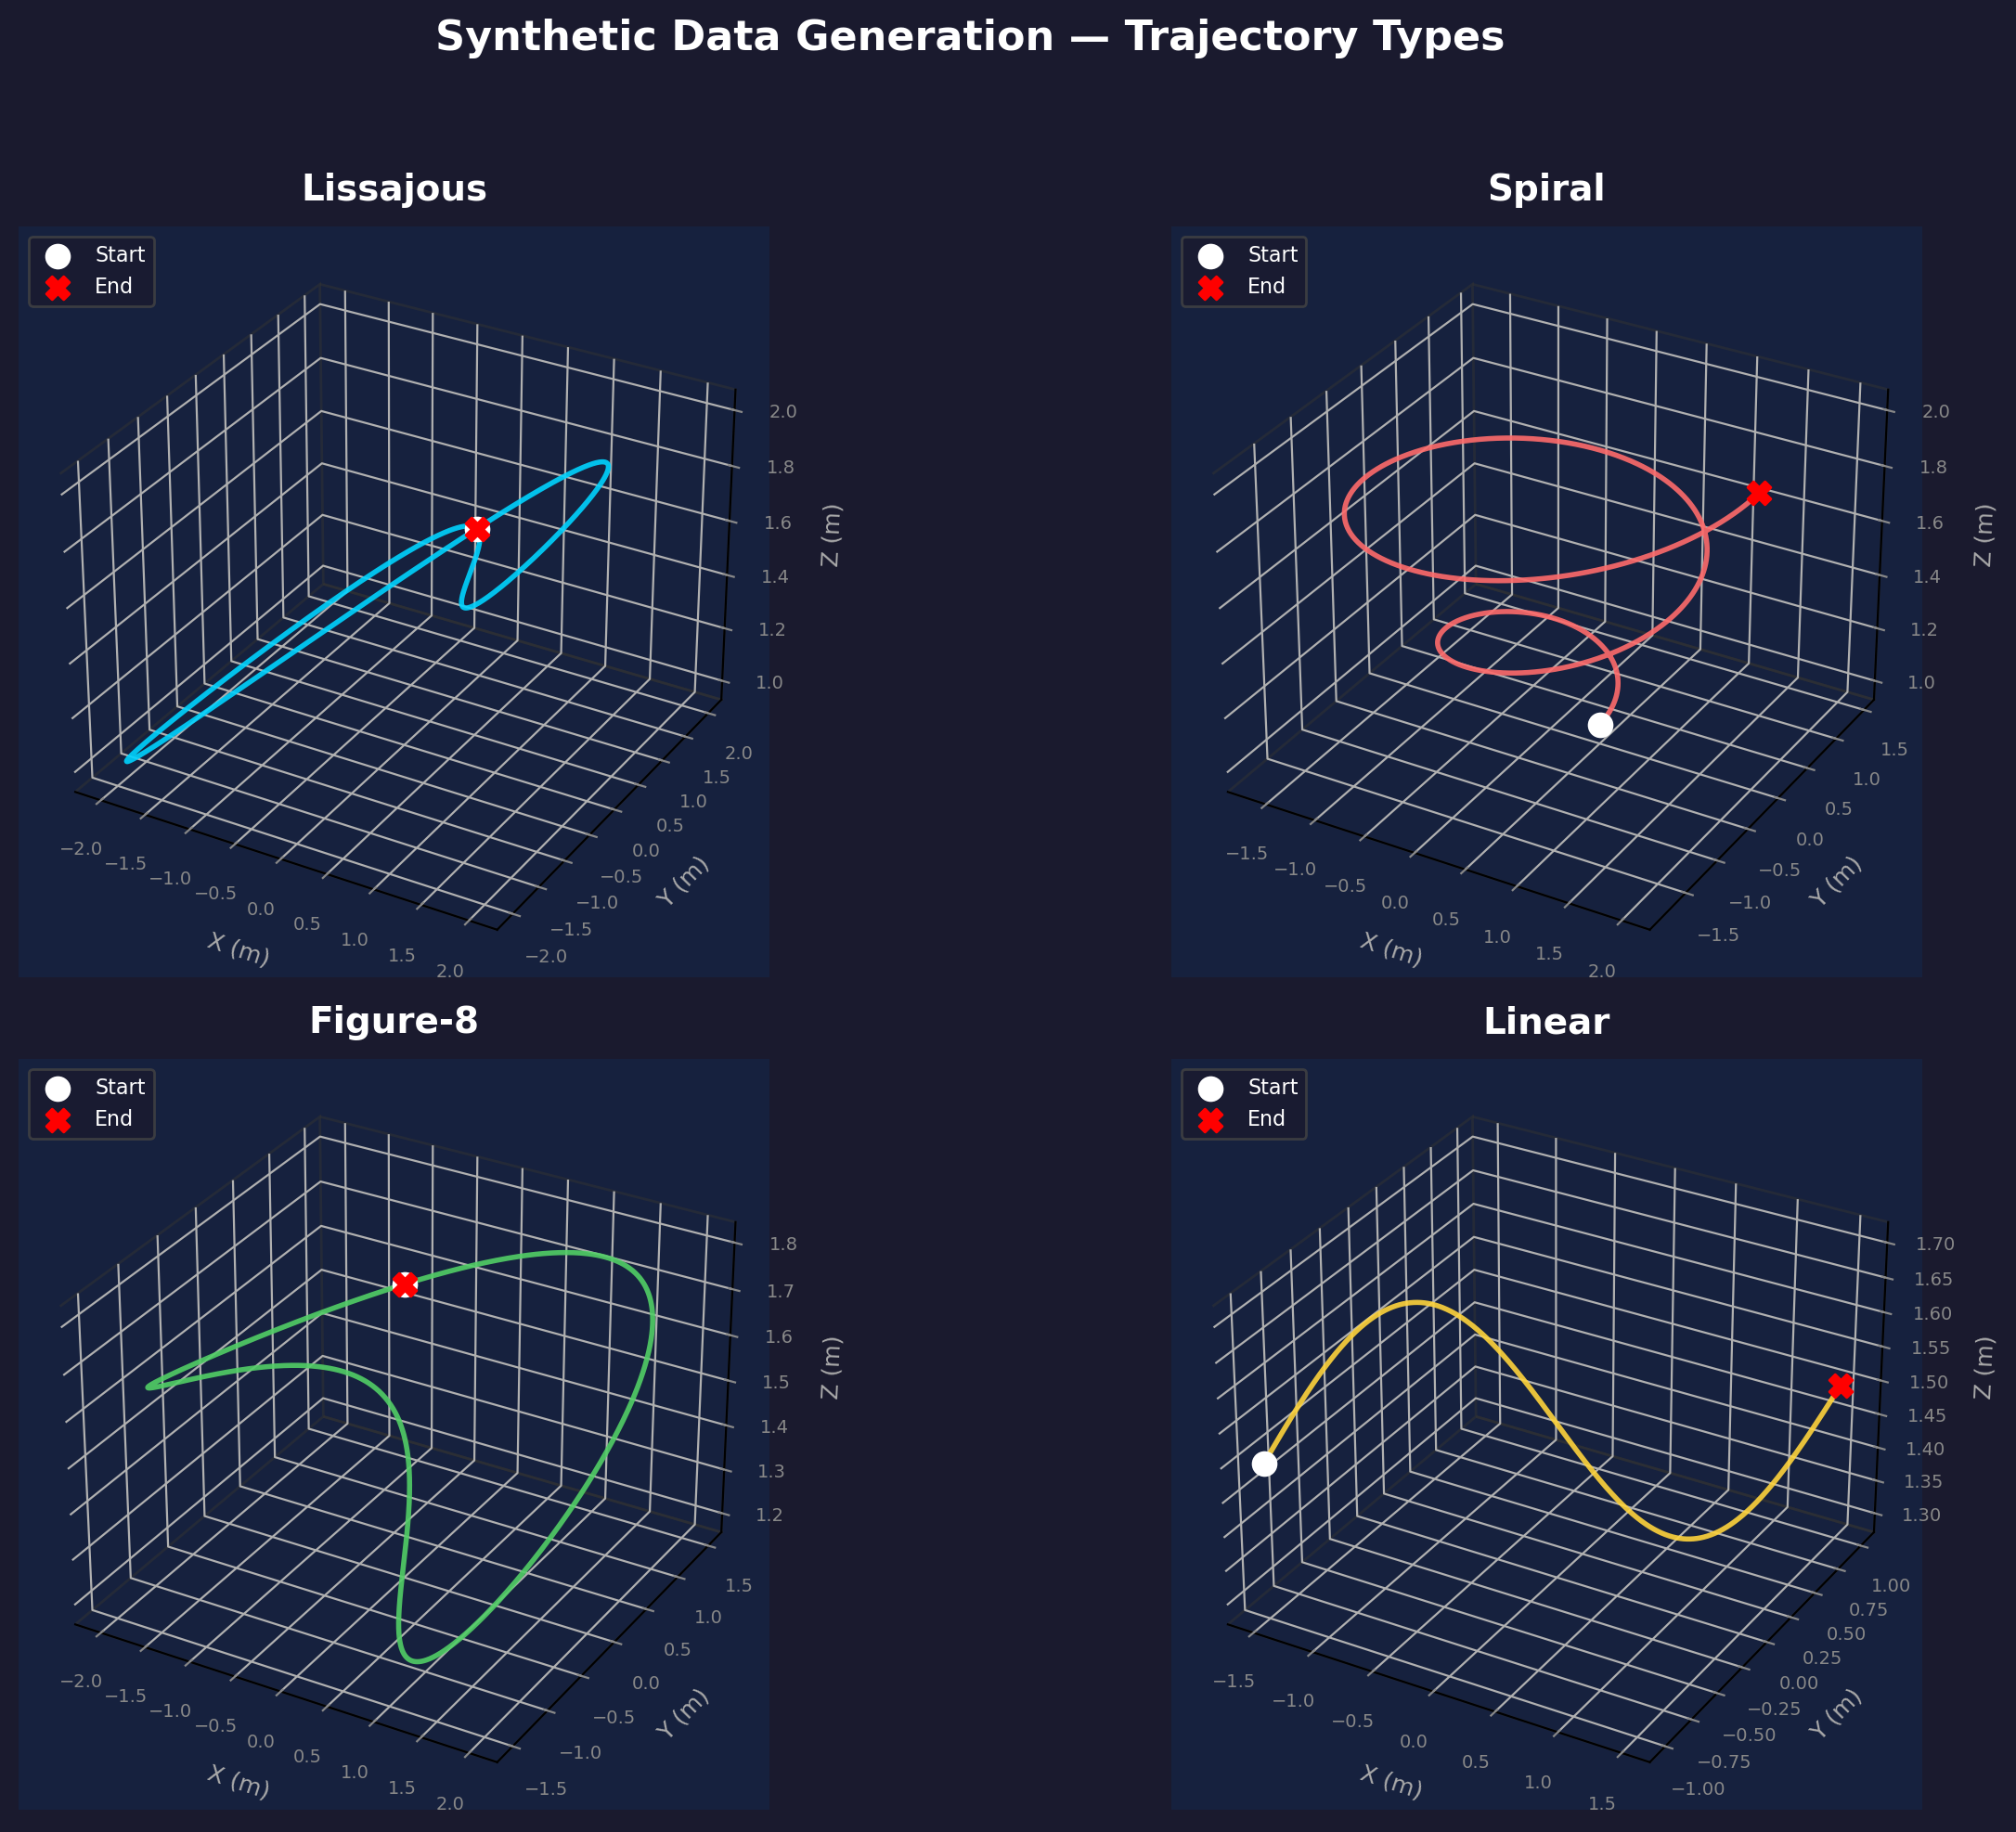
\includegraphics[width=\columnwidth]{figures/trajectory_types.png}
    \caption{The four synthetic trajectory families used for data generation: Lissajous, Spiral, Figure-8, and Linear. White circles indicate start positions; red crosses indicate end positions. Training uses the first three types; the linear trajectory is reserved for validation to test generalization to unseen motion patterns.}
    \label{fig:traj_types}
\end{figure}

\textbf{IMU Simulation.} Ideal accelerometer and gyroscope signals are derived from trajectory derivatives and corrupted with realistic noise following the OysterSim mid-accuracy IMU profile, including bias instability and random walk. IMU is sampled at 1000~Hz.

\textbf{Data Splits.} Training: 3 trajectory types (figure-8, spiral, Lissajous) $\times$ 28 textures = 64 sequences after quality filtering. Validation: 1 unseen trajectory type (linear) $\times$ 20 sequences. Test: figure-8 with unseen texture combinations $\times$ 22 sequences.

\begin{figure}[t]
    \centering
    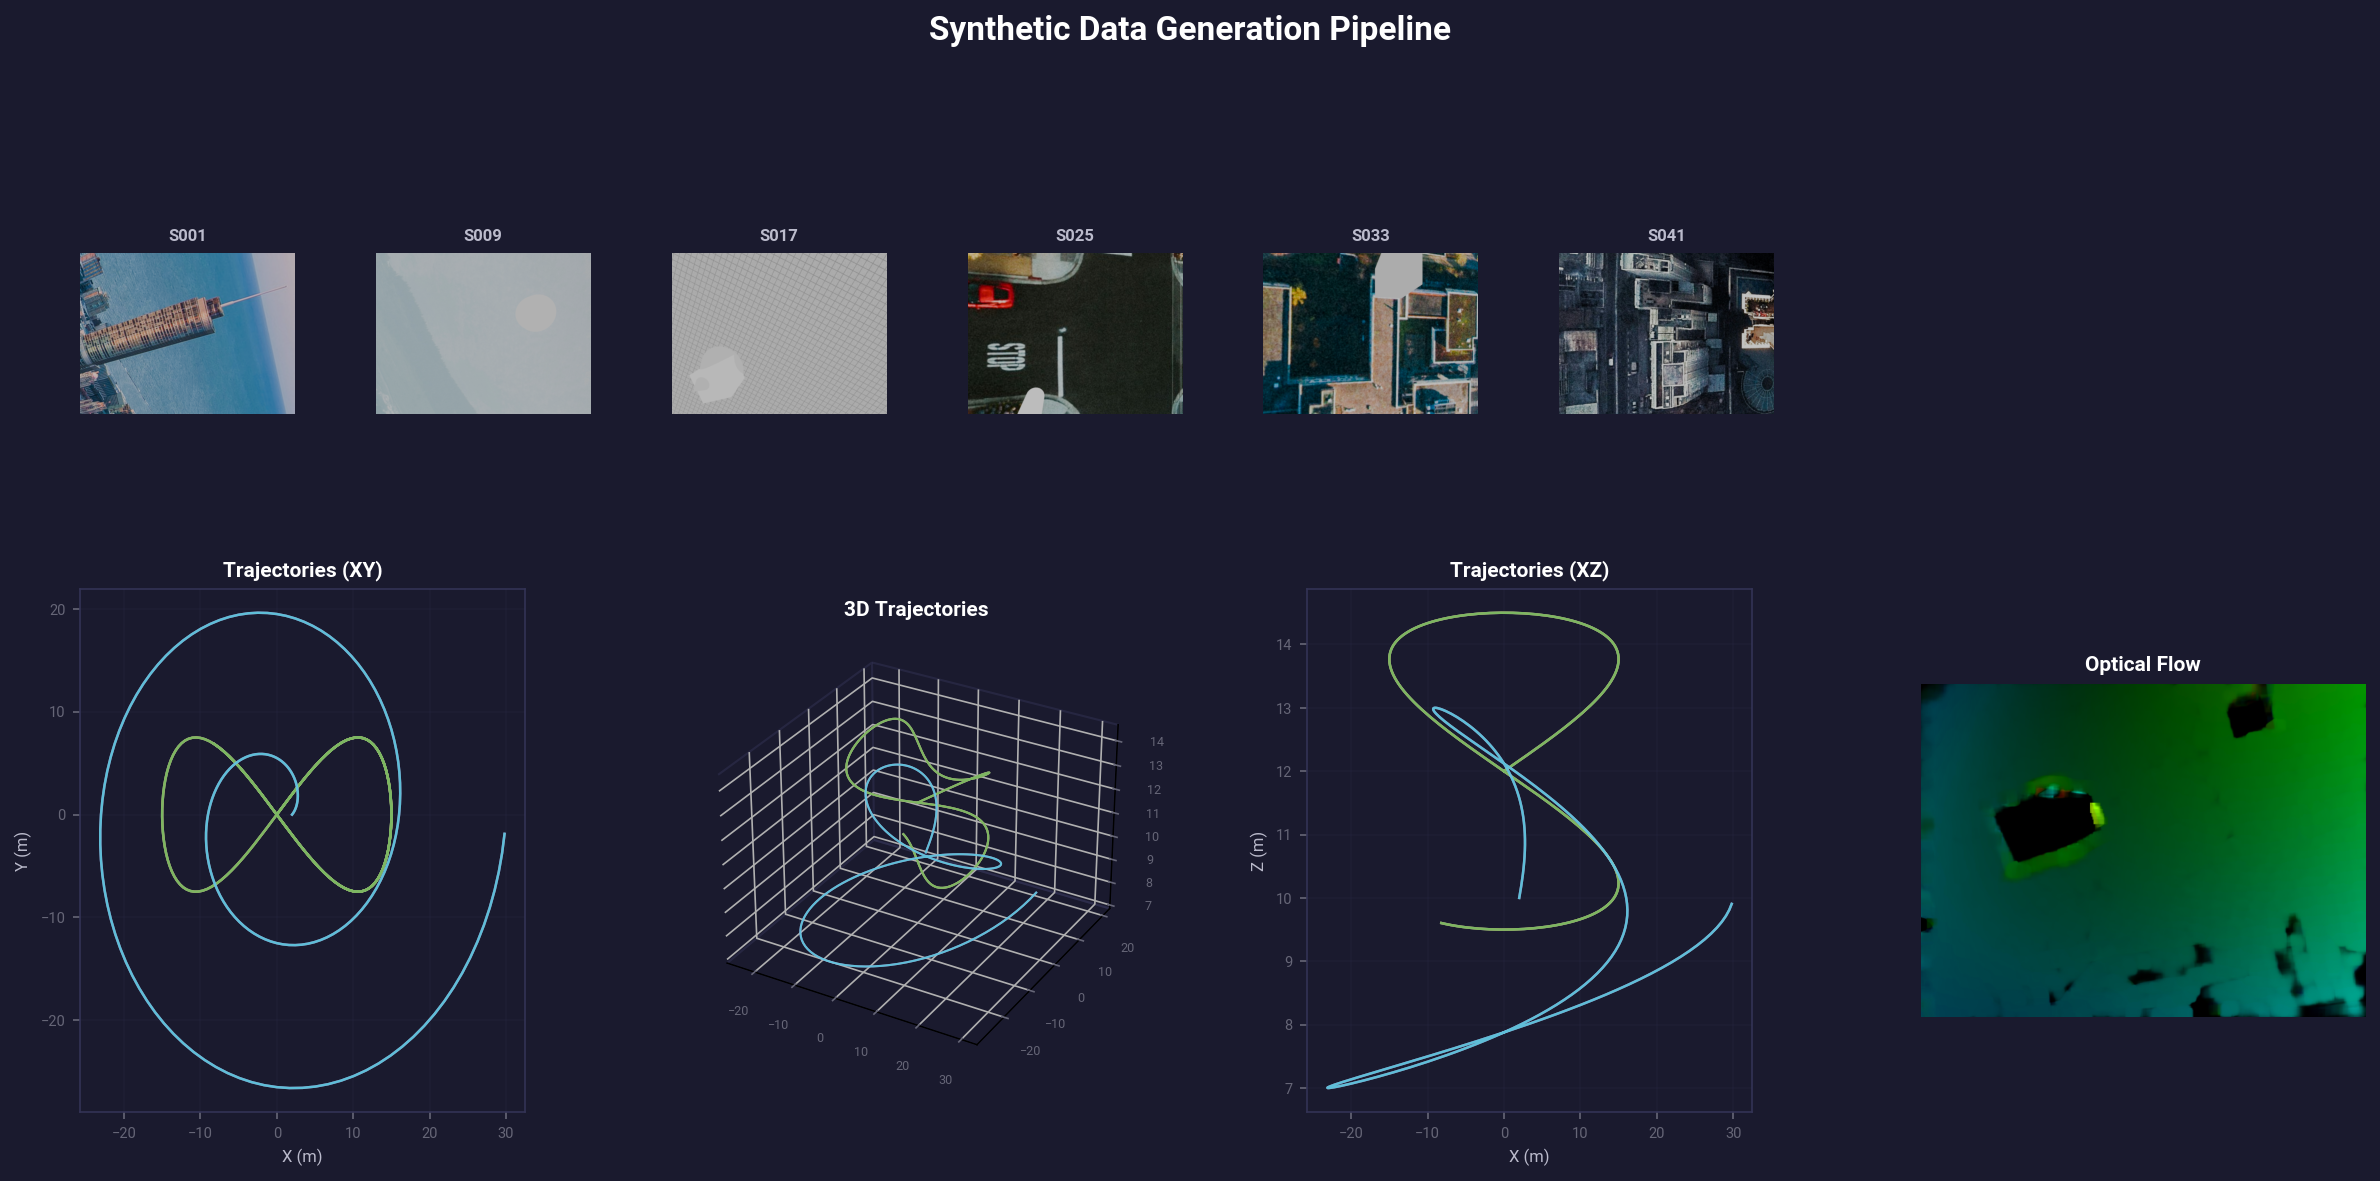
\includegraphics[width=\columnwidth]{visualizations/fig10_data_generation.png}
    \caption{Synthetic data generation pipeline: sample rendered images across textures (top) and generated trajectories with precomputed optical flow (bottom).}
    \label{fig:data_pipeline}
\end{figure}

\subsection{Network Architecture}

We implement three model variants sharing common encoder designs (Fig.~\ref{fig:architecture}).

\textbf{Visual Encoder.} We compare two designs: (a) a 4-layer CNN (735K params) trained from scratch, and (b) a ResNet-18~\cite{he2016} backbone pretrained on ImageNet (11.4M params) with the first convolution modified for 6-channel input (stacked image pair).

\textbf{IMU Encoder.} A 2-layer bidirectional LSTM processes the IMU sequence ($B \times 100 \times 6$). The concatenated forward/backward hidden states produce a 256-dimensional feature vector with LayerNorm.

\textbf{FiLM Fusion.} Instead of concatenating visual and IMU features, the IMU encoder output generates per-channel scale $\gamma$ and shift $\beta$ that modulate visual features:
\begin{equation}
    \mathbf{v}_{mod} = \gamma(\mathbf{f}_{imu}) \odot \mathbf{v} + \beta(\mathbf{f}_{imu})
\end{equation}
where $\gamma, \beta \in \mathbb{R}^{256}$ are produced by learned linear projections from the 256-d IMU feature. A soft gate $\alpha = \sigma(\text{MLP}([\mathbf{v}_{mod}; \mathbf{f}_{imu}]))$ learns to weight the modalities:
\begin{equation}
    \mathbf{f}_{fused} = \alpha \cdot \mathbf{v}_{mod} + (1 - \alpha) \cdot \mathbf{f}_{imu}
\end{equation}

\textbf{Pose Regression.} The fused feature passes through FC layers (256$\to$128$\to$64) with PReLU and dropout to predict position ($\Delta x, \Delta y, \Delta z$) and rotation (unit quaternion $q_x, q_y, q_z, q_w$).

\subsection{Model Variants}

We implement and evaluate three model families, each isolating a different sensory modality:

\textbf{DeepVO (Visual Odometry).} Uses only the visual encoder to predict relative pose from consecutive image pairs. The stacked 6-channel input (frame $t$ concatenated with frame $t+1$) is processed by either the 4-layer CNN or the pretrained ResNet-18. This model tests whether visual features alone are sufficient for odometry on our synthetic scenes. Following DeepVO~\cite{wang2017}, we use no temporal LSTM---each image pair independently predicts a relative pose.

\textbf{DeepIO (Inertial Odometry).} Uses only the IMU encoder to predict relative pose from inertial measurements between consecutive camera frames. The bidirectional LSTM processes 100 IMU samples (6-DoF: 3-axis gyroscope + 3-axis accelerometer) at 1000~Hz spanning the 0.1s inter-frame interval. This model tests whether IMU alone---with realistic noise from the OysterSim profile---can estimate ego-motion. DeepIO serves as a lower bound for the fused model; if VIO cannot outperform IO, the visual branch is not contributing.

\textbf{DeepVIO (Visual-Inertial Odometry).} Fuses both modalities. We compare two fusion strategies: (a) naive concatenation of visual and IMU feature vectors (512-d $\to$ FC heads), and (b) FiLM conditioning with soft gating as described above. The fused model should ideally outperform both individual modalities by leveraging complementary information---visual features for position estimation and IMU for rotation and short-term dynamics.

\subsection{Loss Function}

We use a combined L1 position loss and geodesic quaternion rotation loss:
\begin{equation}
    \mathcal{L} = \lambda_p \|\mathbf{p} - \hat{\mathbf{p}}\|_1 + \lambda_q \cdot 2\arccos(|\mathbf{q} \cdot \hat{\mathbf{q}}|)
\end{equation}
with $\lambda_p = \lambda_q = 1.0$.

\subsection{Two-Stage Training}

To address the modality imbalance problem, we propose a two-stage training strategy:

\textbf{Stage 1: Visual Pretraining.} Train the ResNet-18 visual encoder independently as a DeepVO model (50 epochs, LR=$5 \times 10^{-4}$).

\textbf{Stage 2: Frozen Visual + Fusion Training.} Load pretrained visual weights into the FiLM model, freeze the visual encoder, and train only the IMU encoder, FiLM layers, gate, and pose heads (10 epochs, LR=$5 \times 10^{-4}$).

\textbf{Stage 3: Joint Finetuning.} Unfreeze all parameters and finetune end-to-end with reduced learning rate (LR=$1 \times 10^{-4}$, early stopping with patience 15).

This prevents the IMU from dominating early in training, forcing the fusion layers to learn to \textit{use} the pretrained visual features.

% ======================================================================
\section{Experiments and Results}
% ======================================================================

\subsection{Data Quality Diagnosis}

\begin{figure}[t]
    \centering
    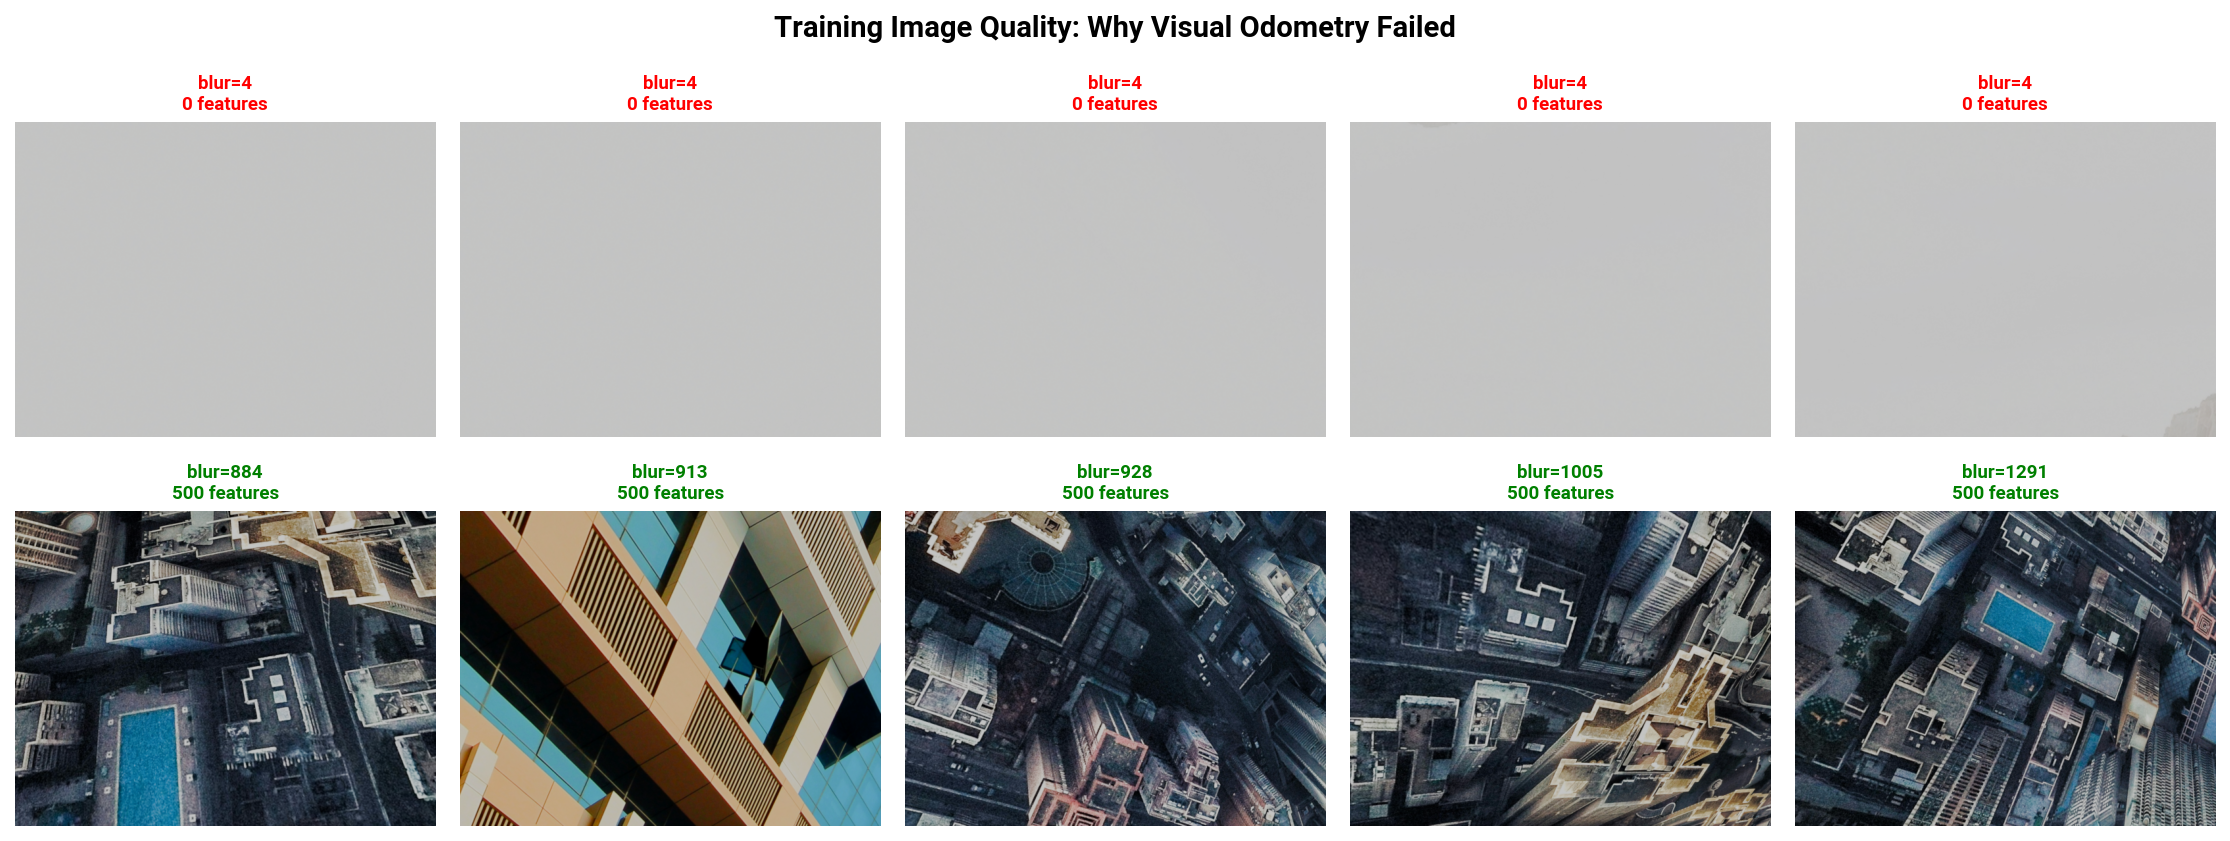
\includegraphics[width=\columnwidth]{visualizations/fig1_image_quality_grid.png}
    \caption{Original dataset quality: top row shows unusable sequences (blur $<$ 20, 0 features), bottom row shows usable sequences. 22\% of training data was essentially blank.}
    \label{fig:data_quality}
\end{figure}

Our initial training revealed that the combined model performed \textit{worse} than vision-only (Table~\ref{tab:main_results}). Systematic analysis revealed the root cause: 54\% of training images had insufficient texture for visual odometry (Fig.~\ref{fig:data_quality}). We measured image sharpness using Laplacian variance~\cite{pech2000}, finding that 7 of 22 source textures produced near-uniform renders when viewed from 12m altitude. After removing bad textures, adding procedural textures, inserting 3D scene objects, and filtering sequences with blur score $<30$, all remaining images exceeded the usable threshold.

\subsection{Baseline Results}

Table~\ref{tab:main_results} shows the progressive improvement across data fixes and architectural changes.

\begin{table}[t]
\centering
\caption{Test Loss Across All Experiments}
\label{tab:main_results}
\begin{tabular}{@{}lccc@{}}
\toprule
\textbf{Model} & \textbf{Test Loss} & \textbf{Pos} & \textbf{Rot} \\
\midrule
\multicolumn{4}{l}{\textit{Original Dataset (54\% unusable images)}} \\
DeepVO (CNN) & 0.3017 & 0.2815 & 0.0202 \\
DeepIO (LSTM) & 0.5430 & 0.5321 & 0.0109 \\
DeepVIO (concat) & 0.5129 & 0.4970 & 0.0159 \\
\midrule
\multicolumn{4}{l}{\textit{Curated Dataset (100\% usable, 3D objects)}} \\
DeepVO (CNN) & 0.1822 & 0.1622 & 0.0200 \\
DeepIO (LSTM) & 0.2437 & 0.2211 & 0.0226 \\
DeepVIO (concat) & 0.2055 & 0.1868 & 0.0187 \\
\midrule
\multicolumn{4}{l}{\textit{V2 Models (ResNet-18 + FiLM)}} \\
DeepVO\_V2 (ResNet-18) & 0.0295 & 0.0269 & 0.0026 \\
DeepVIO FiLM (one-shot) & 0.1331 & 0.1194 & 0.0137 \\
\textbf{DeepVIO FiLM (two-stage)} & \textbf{0.0237} & \textbf{0.0197} & \textbf{0.0040} \\
\bottomrule
\end{tabular}
\end{table}

\subsection{DeepVO: Visual Odometry Analysis}

The visual-only model shows the clearest progression across our improvements. On the original dataset with featureless images, the CNN-based DeepVO achieved a test loss of 0.3017 with the model training stably for 21 epochs---the best generalization among all baseline models. This is because visual features, when present, provide strong position cues through apparent motion of texture on the ground plane.

After dataset curation, the same CNN architecture improved to 0.1822 (40\% reduction), confirming that data quality was the primary bottleneck. Replacing the CNN with a pretrained ResNet-18 further reduced test loss to 0.0295 (90\% total reduction), with the model training for a full 50 epochs without early stopping. The ResNet-18 DeepVO achieves the lowest rotation error (0.0026) of any model, indicating that pretrained features excel at capturing fine orientation changes from visual parallax.

On trajectory evaluation (Fig.~\ref{fig:all_models}), DeepVO achieves the best ATE on seen trajectory types: 1.2--1.8m on figure-8 test sequences and 1.5m on spiral. However, on the unseen linear trajectory, ATE degrades to 27--32m, suggesting the model learns trajectory-shape priors rather than general visual odometry.

\subsection{DeepIO: Inertial Odometry Analysis}

The IMU-only model exhibits fundamentally different training dynamics. DeepIO converges extremely fast---best validation at epoch 2--3 on both datasets---then immediately overfits (train loss 0.07 vs val loss 0.36 by epoch 13). This is because IMU sequences within the same trajectory family are highly correlated, allowing the LSTM to memorize motion patterns.

On the original dataset, DeepIO achieves low rotation error (0.0109) but high position error (0.5321), reflecting that gyroscope integration is inherently more accurate than double-integration of accelerometers for position. On the curated dataset, DeepIO improves to 0.2437 test loss, though this improvement comes from the dataset restructuring (different train/test split) rather than visual quality changes.

Critically, DeepIO produces \textit{constant} ATE across test sequences (10.61m for all three), confirming it memorizes an average motion pattern rather than responding to per-sequence input. On the unseen linear trajectory, ATE jumps to 48.1m---the worst of all models---because the learned spiral/figure-8 priors are entirely wrong for straight-line motion.

\subsection{DeepVIO: Visual-Inertial Fusion Analysis}

\begin{figure}[t]
    \centering
    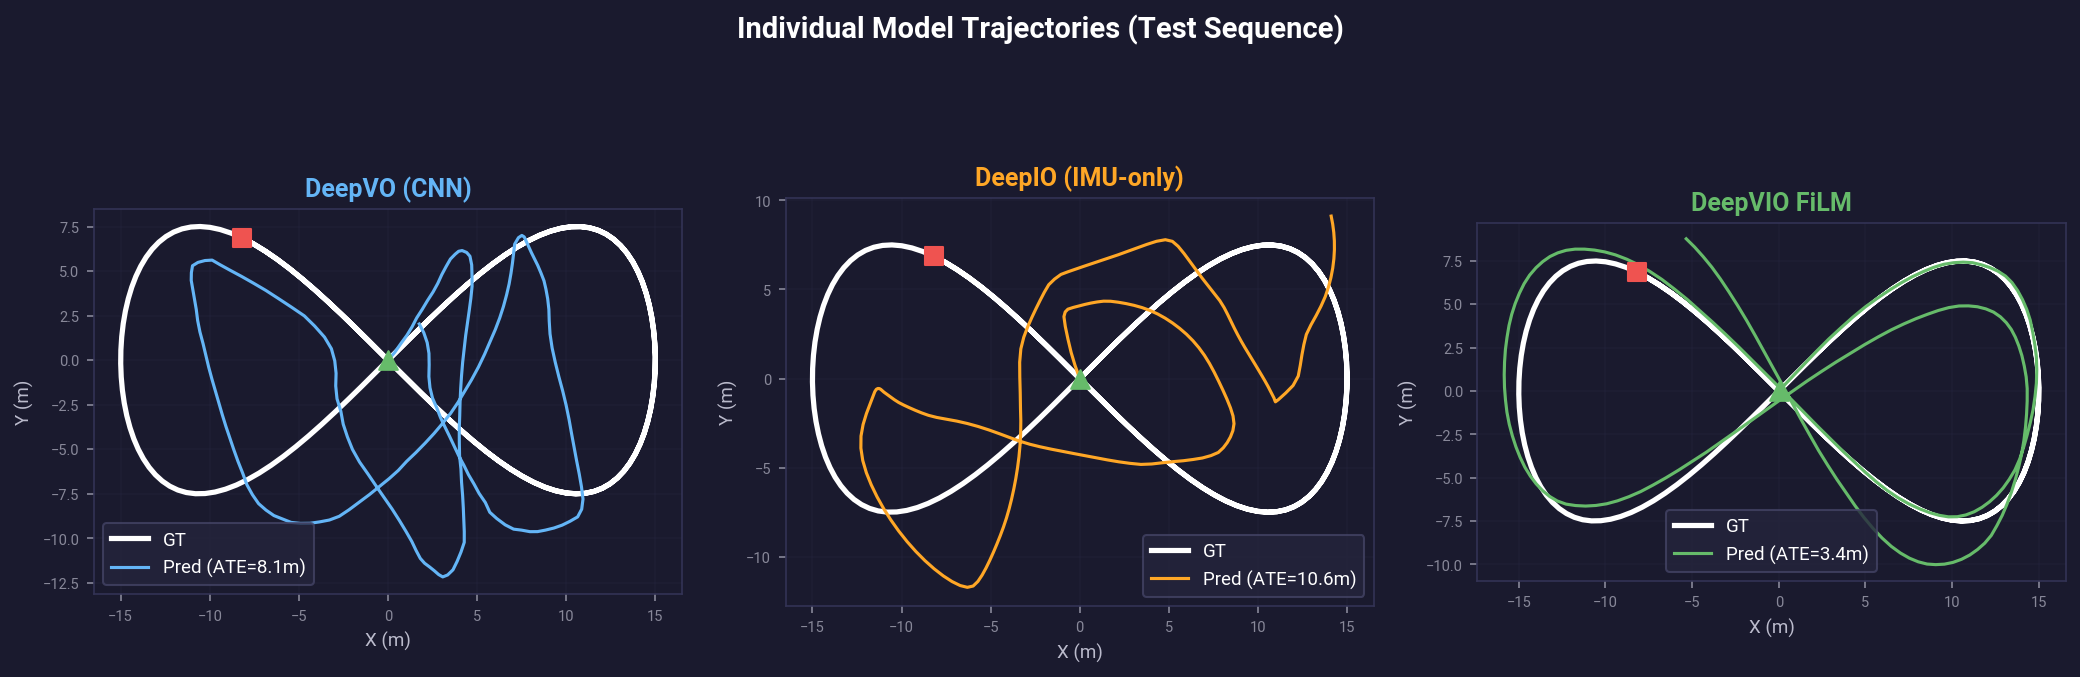
\includegraphics[width=\columnwidth]{visualizations/fig21_vo_io_vio_individual.png}
    \caption{Individual model trajectories on a test sequence: DeepVO (CNN) tracks the shape but drifts, DeepIO predicts a fixed pattern regardless of input, DeepVIO FiLM (two-stage) achieves the best shape fidelity.}
    \label{fig:all_models}
\end{figure}

The fusion results reveal the modality imbalance problem most clearly. With naive concatenation on the original dataset, DeepVIO (test loss 0.5129) performs \textit{worse} than DeepVO alone (0.3017)---the fusion actively degrades performance because the IMU branch dominates gradient flow and suppresses visual learning. The best epoch is always 1, indicating the model never learns meaningful fusion.

On the curated dataset, concatenation-based DeepVIO improves to 0.2055 but still underperforms DeepVO (0.1822). The FiLM fusion with one-shot training achieves 0.1331 but the gate analysis reveals vision is suppressed ($\alpha = 0.07\text{--}0.18$).

Only with two-stage training does the fused model finally outperform the visual-only model: test loss 0.0237 vs 0.0295, with a balanced gate ($\alpha = 0.39\text{--}0.47$). This represents the first successful visual-inertial fusion in our experiments and validates the combination of FiLM conditioning and staged training.

\begin{table}[t]
\centering
\caption{Complete ATE Results --- All Models (meters)}
\label{tab:ate_all}
\begin{tabular}{@{}lcc@{}}
\toprule
\textbf{Model} & \textbf{Test Avg} & \textbf{Val Avg (unseen)} \\
\midrule
DeepVO (CNN) & 6.6 & 33.8 \\
DeepIO (LSTM) & 10.6 & 48.1 \\
DeepVIO (Concat) & 17.1 & 41.5 \\
DeepVO (ResNet-18) & \textbf{1.5} & 29.9 \\
DeepVIO FiLM (two-stage) & 3.5 & \textbf{31.3} \\
\bottomrule
\end{tabular}
\end{table}

\subsection{Modality Imbalance and Gate Analysis}

\begin{figure}[t]
    \centering
    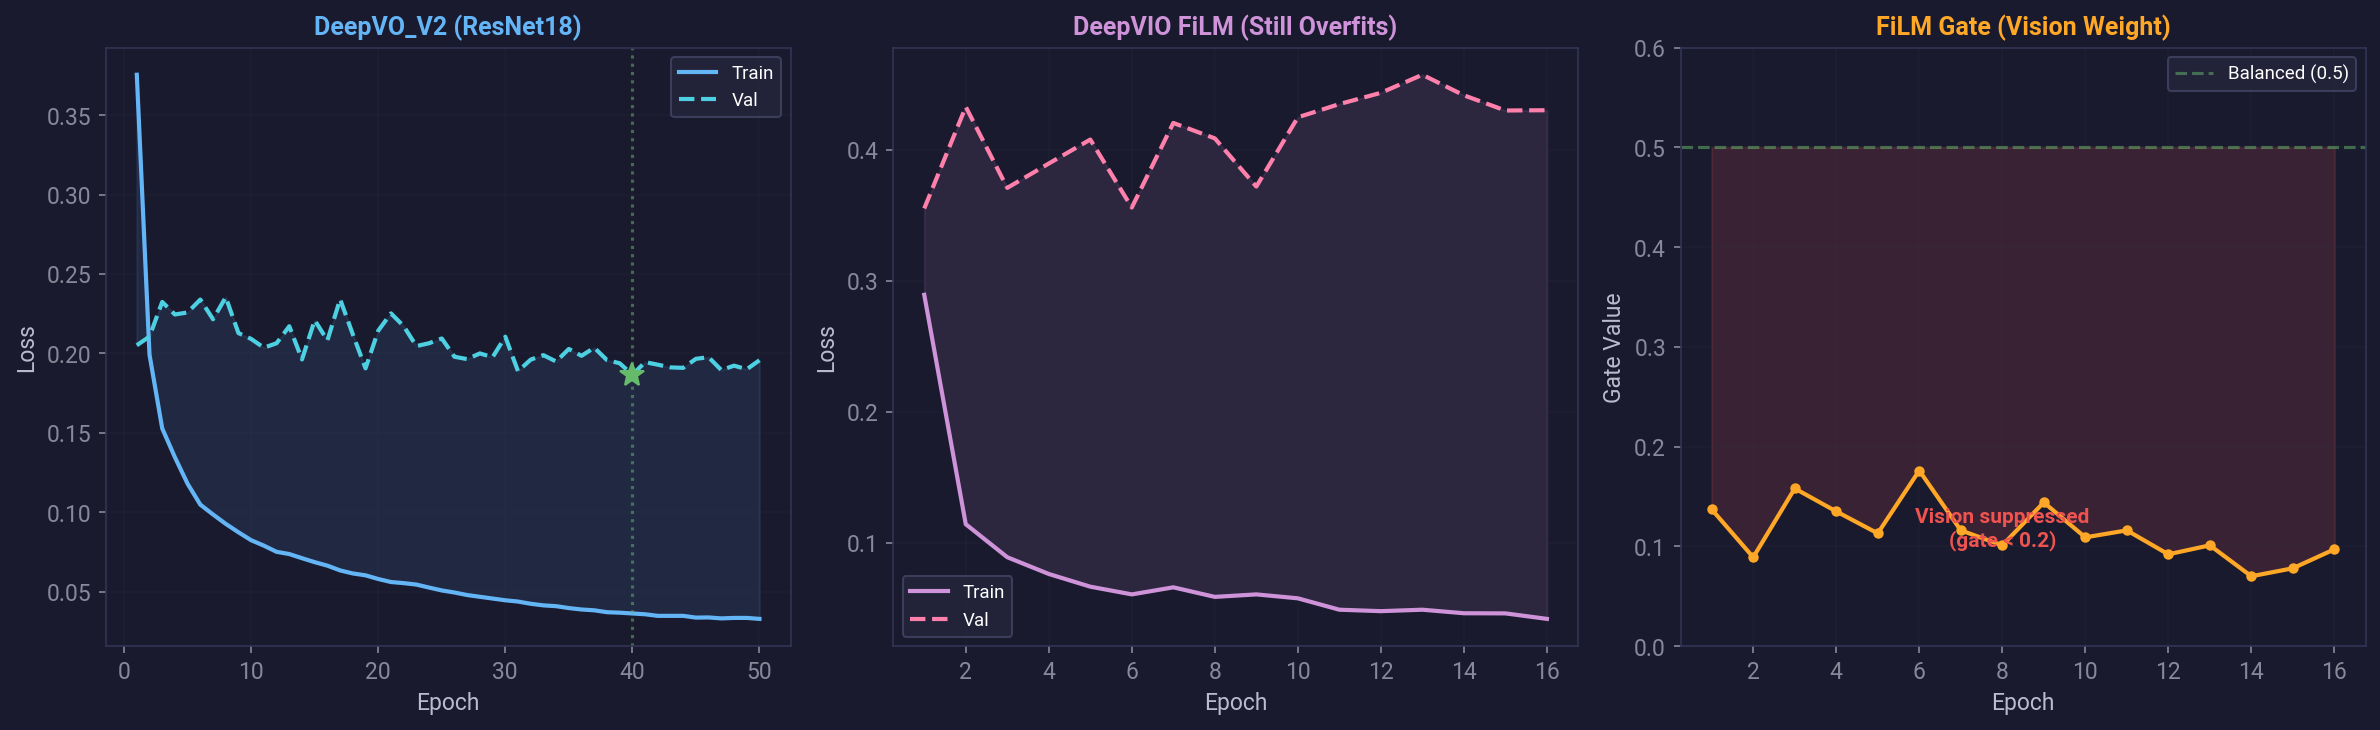
\includegraphics[width=\columnwidth]{visualizations/fig12_v2_training_curves.png}
    \caption{V2 training dynamics. Left: ResNet-18 visual model. Center: FiLM one-shot (overfits). Right: FiLM gate values---one-shot training suppresses vision ($\alpha < 0.2$).}
    \label{fig:training_curves}
\end{figure}

The soft gate reveals the modality imbalance problem (Fig.~\ref{fig:training_curves}, right). With one-shot training, the gate drops to $\alpha = 0.07\text{--}0.18$, meaning vision contributes only 7--18\% to the fused representation. With two-stage training, the gate stabilizes at $\alpha = 0.39\text{--}0.47$, achieving near-balanced fusion. This confirms that pretraining the visual encoder separately prevents IMU from dominating.

\subsection{Trajectory Evaluation}

\begin{figure}[h]
\centering
\setlength{\tabcolsep}{3pt}
\begin{tabular}{ccc}
  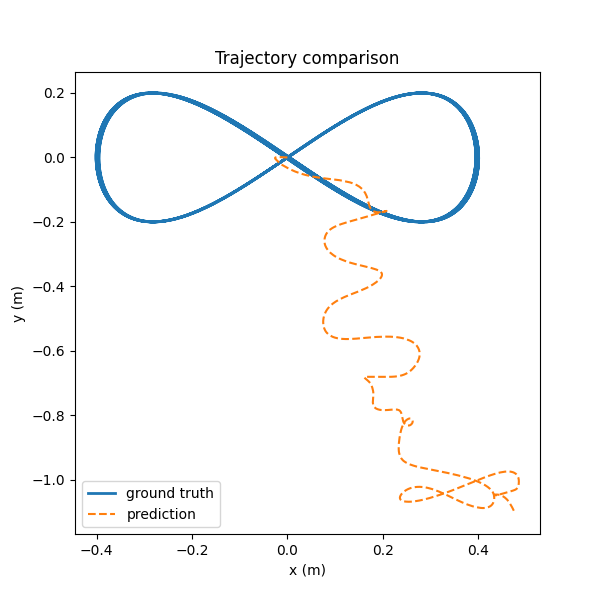
\includegraphics[width=0.31\columnwidth]{figures/imu_trajectory.png}    &
  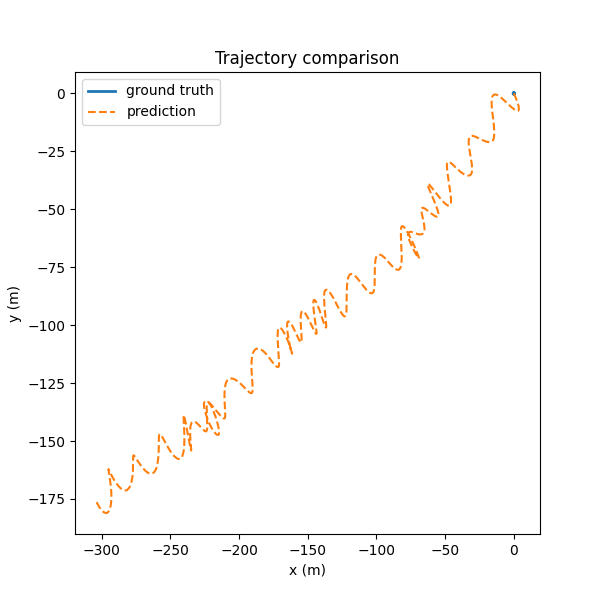
\includegraphics[width=0.31\columnwidth]{figures/vision_trajectory.png} &
  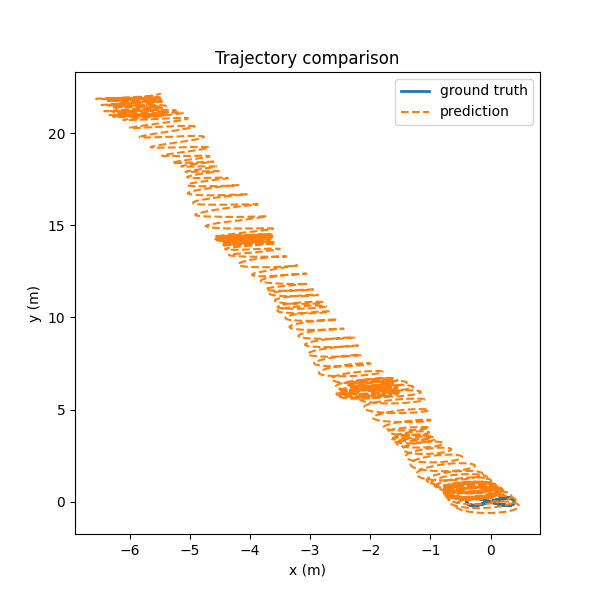
\includegraphics[width=0.31\columnwidth]{figures/vio_trajectory.png}    \\[2pt]
  {\small (a) DeepIO} & {\small (b) DeepVO} & {\small (c) DeepVIO}        \\
\end{tabular}
\caption{Predicted vs.\ ground-truth trajectories for each modality. (a)~DeepIO memorizes an average motion pattern regardless of input. (b)~DeepVO captures trajectory shape but accumulates drift. (c)~DeepVIO (FiLM two-stage) achieves the best shape fidelity by fusing both modalities.}
\label{fig:modality_trajectories}
\end{figure}

\begin{figure}[t]
    \centering
    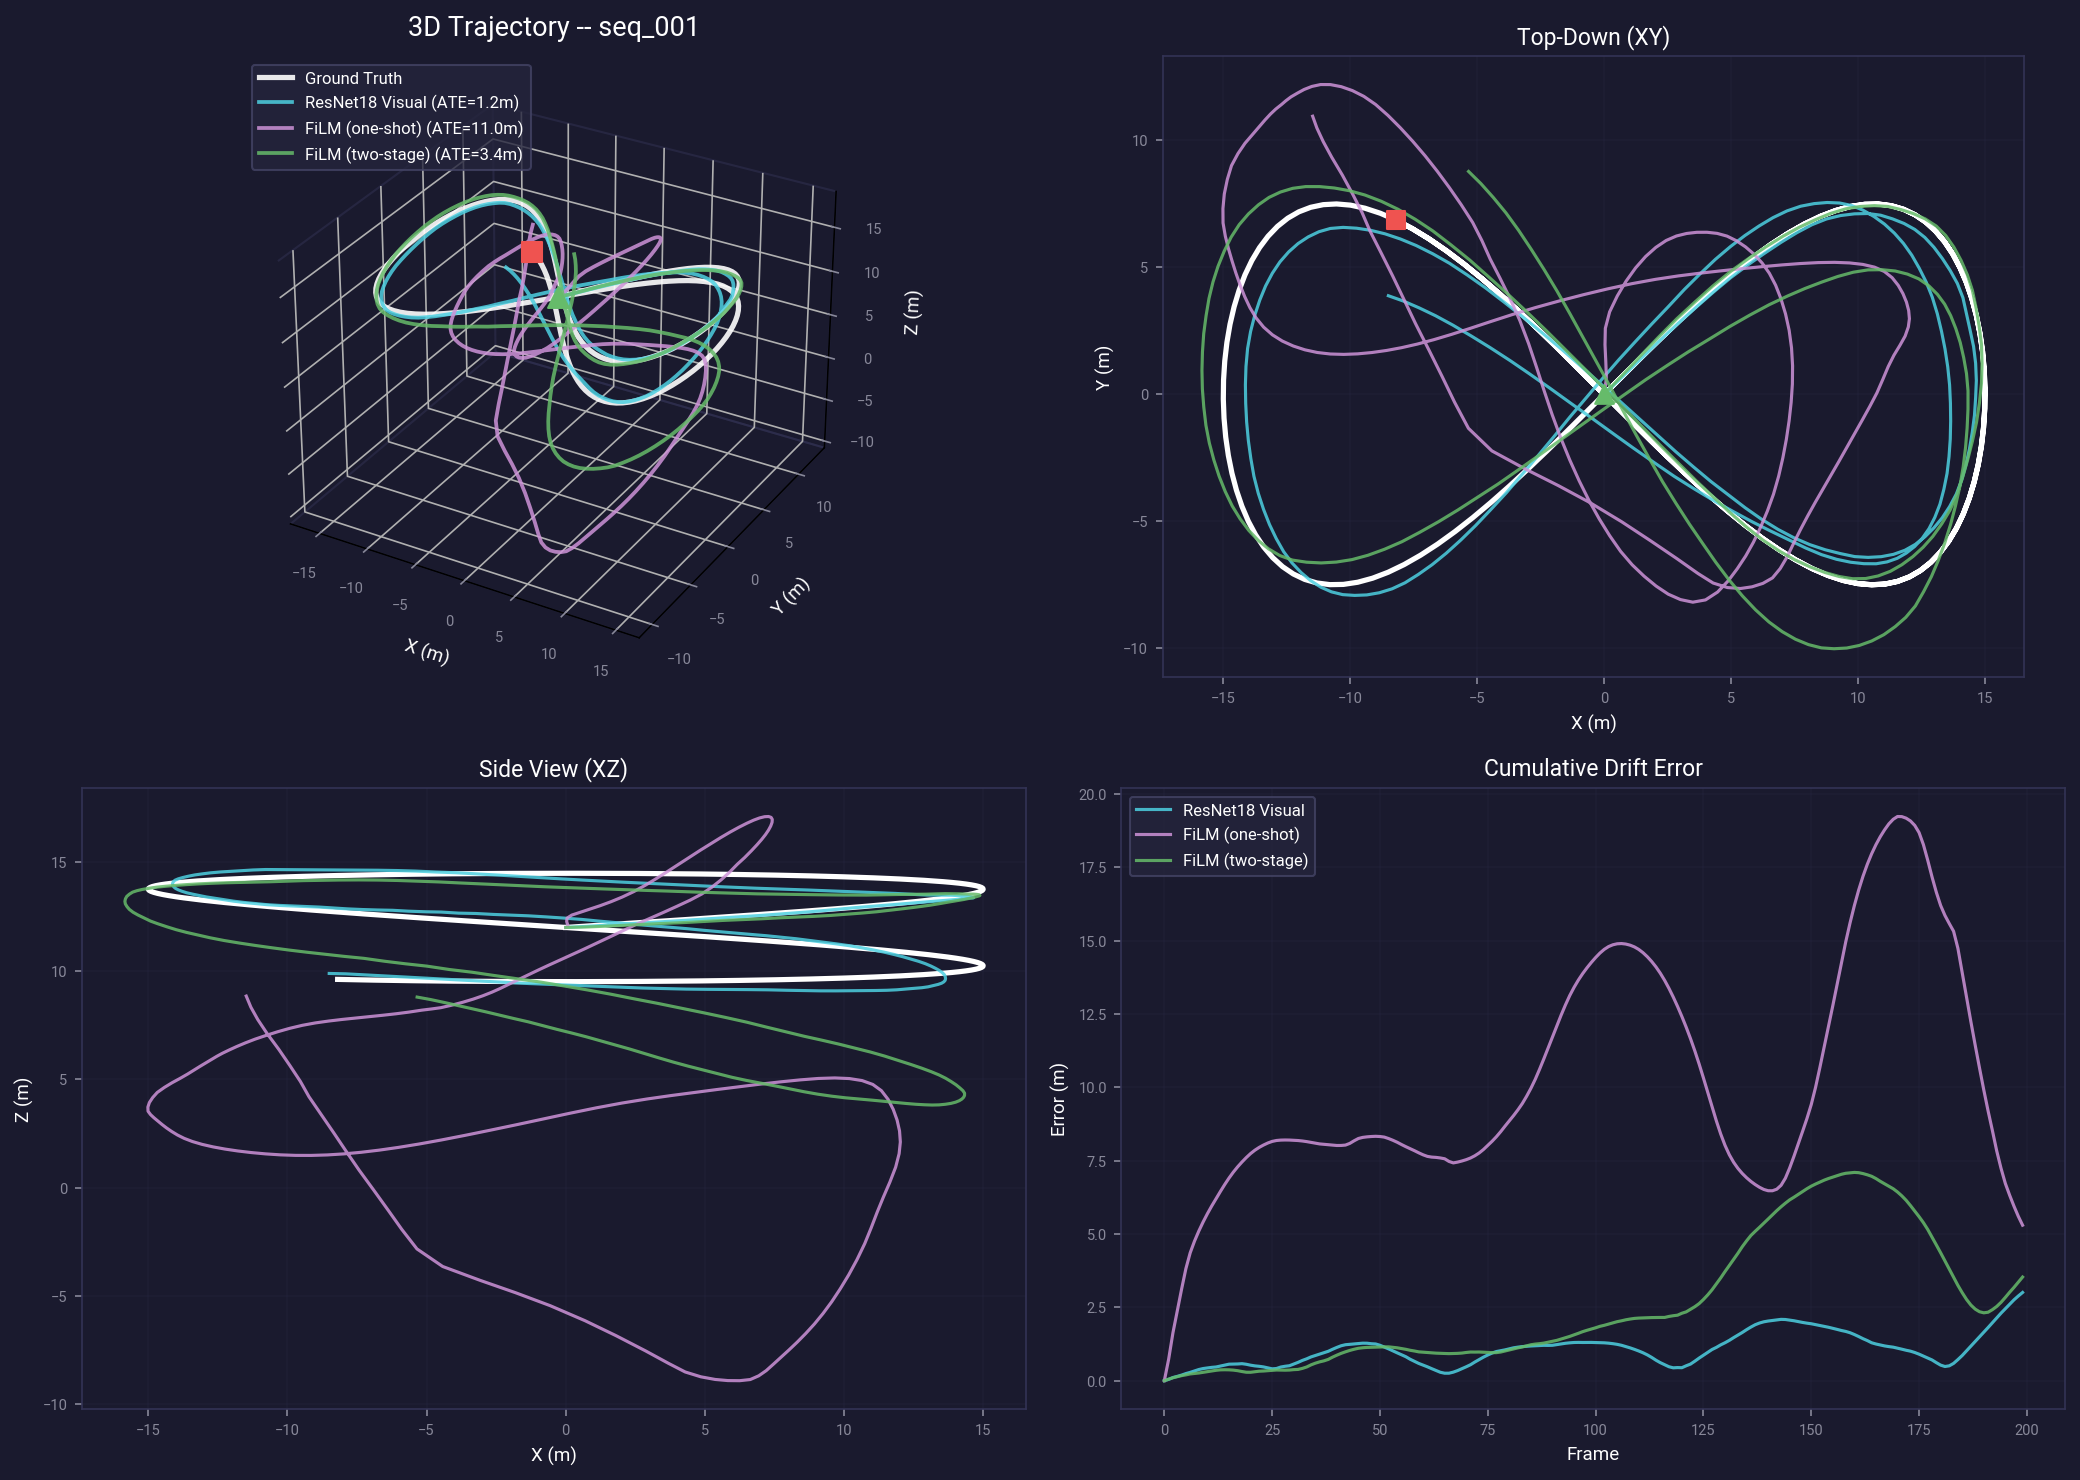
\includegraphics[width=\columnwidth]{visualizations/fig14_v2_trajectory_seq_001.png}
    \caption{3D trajectory reconstruction on test sequence: ground truth (white) vs ResNet-18 (cyan, ATE=1.2m) vs FiLM two-stage (green, ATE=3.4m). Four views: 3D, XY top-down, XZ side, cumulative drift.}
    \label{fig:trajectory}
\end{figure}

Fig.~\ref{fig:trajectory} shows trajectory reconstructions on a test sequence. The ResNet-18 visual model achieves 1.2--1.8m ATE, closely tracking ground truth. The two-stage FiLM model achieves 3.1--4.0m ATE. Table~\ref{tab:ate} summarizes ATE across trajectory types.

\begin{table}[t]
\centering
\caption{Absolute Trajectory Error (m) by Trajectory Type --- All Models}
\label{tab:ate}
\begin{tabular}{@{}lcccccc@{}}
\toprule
\textbf{Traj.} & \textbf{Seen?} & \textbf{VO} & \textbf{IO} & \textbf{VIO} & \textbf{VO-R} & \textbf{FiLM} \\
 & & \textbf{CNN} & \textbf{LSTM} & \textbf{Cat.} & \textbf{Res18} & \textbf{2-stg} \\
\midrule
Fig-8 & Same & 6.6 & 10.6 & 17.1 & \textbf{1.5} & 3.5 \\
Spiral & Yes & --- & --- & --- & \textbf{1.5} & 3.5 \\
Lissajous & Yes & --- & --- & --- & \textbf{3.2} & 3.8 \\
Linear & \textbf{No} & 33.8 & 48.1 & 41.5 & 29.9 & \textbf{31.3} \\
\bottomrule
\end{tabular}
\end{table}

\subsection{Generalization to Unseen Trajectories}

\begin{figure}[t]
    \centering
    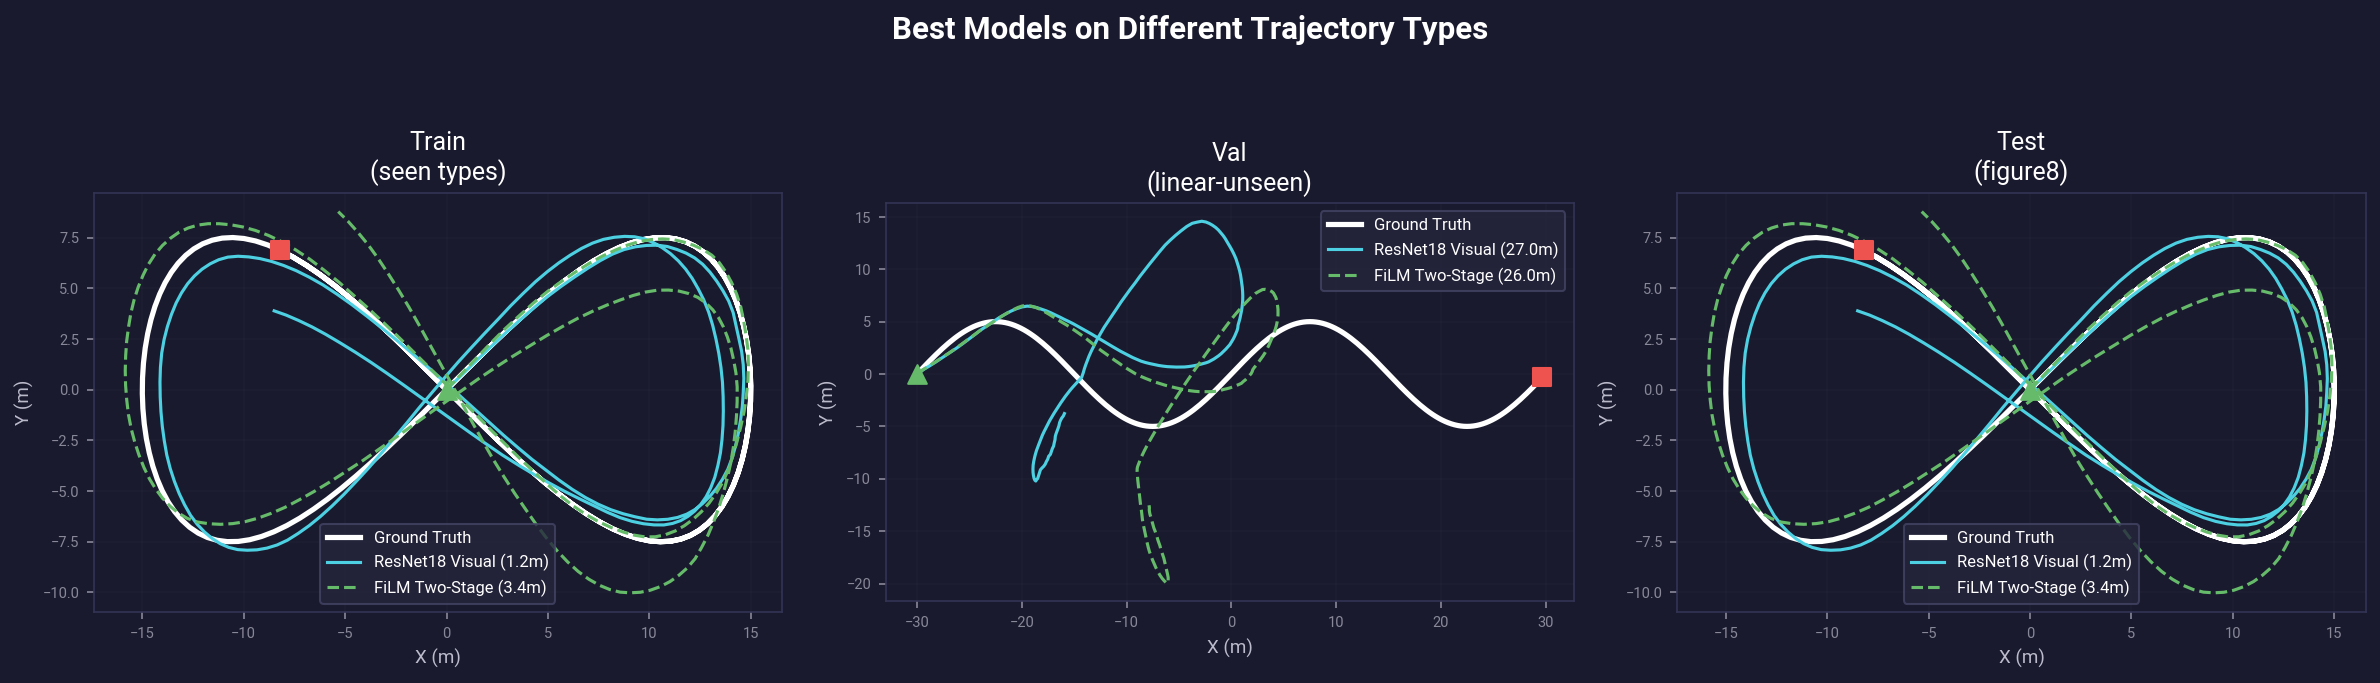
\includegraphics[width=\columnwidth]{visualizations/fig18_cross_trajectory_paths.png}
    \caption{Best model trajectories on seen (train, test) vs unseen (val/linear) trajectory types. Performance degrades significantly on the unseen linear trajectory.}
    \label{fig:generalization}
\end{figure}

On seen trajectory families, both models achieve excellent ATE (1--4m). However, on the unseen linear trajectory type, ATE degrades to 26--36m (Fig.~\ref{fig:generalization}, Table~\ref{tab:ate}). This indicates the models learn trajectory-specific motion priors rather than general odometry, motivating future work with more diverse training trajectories and motion-invariant representations such as optical flow~\cite{wang2021, teed2020}.

\begin{figure}[t]
    \centering
    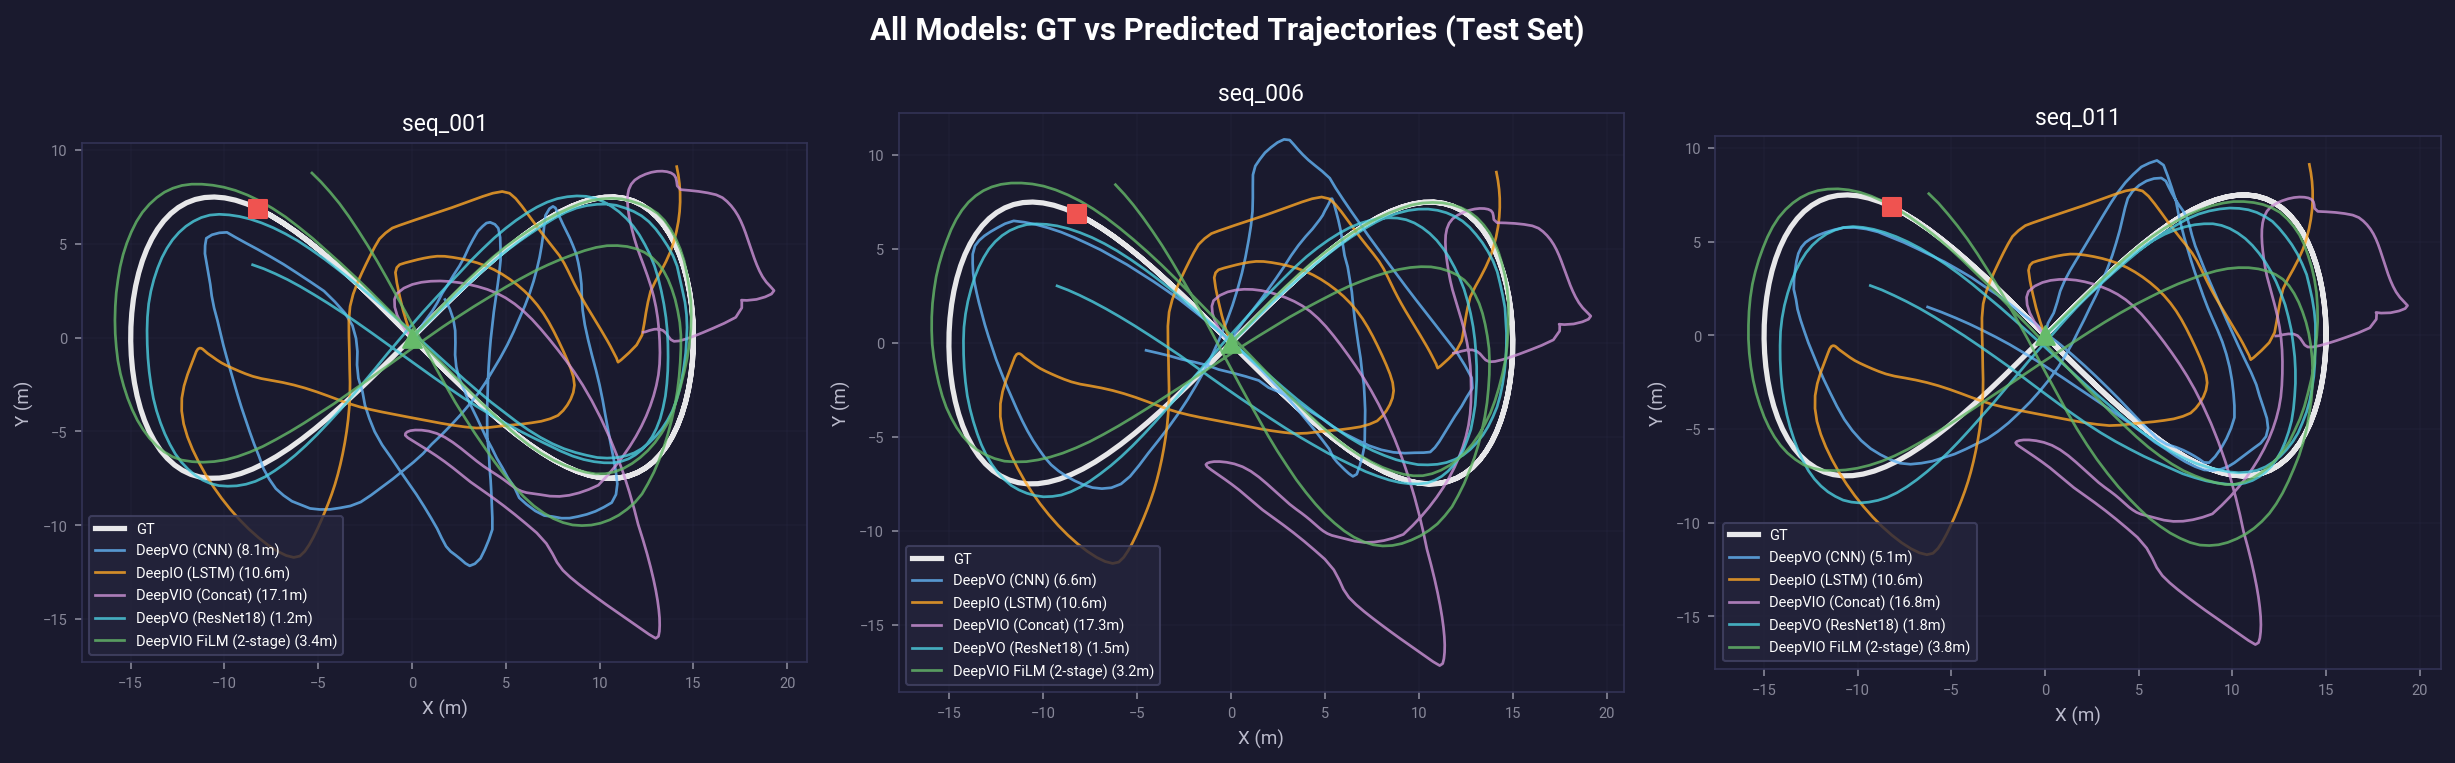
\includegraphics[width=\columnwidth]{visualizations/fig19_all_models_test.png}
    \caption{All five models evaluated on test sequences (top-down XY view). The ResNet-18 visual model (cyan) tracks closest to ground truth, while DeepIO (orange) produces a fixed pattern. The two-stage FiLM model (green) achieves the best combined performance.}
    \label{fig:all_models_test}
\end{figure}

\begin{figure}[t]
    \centering
    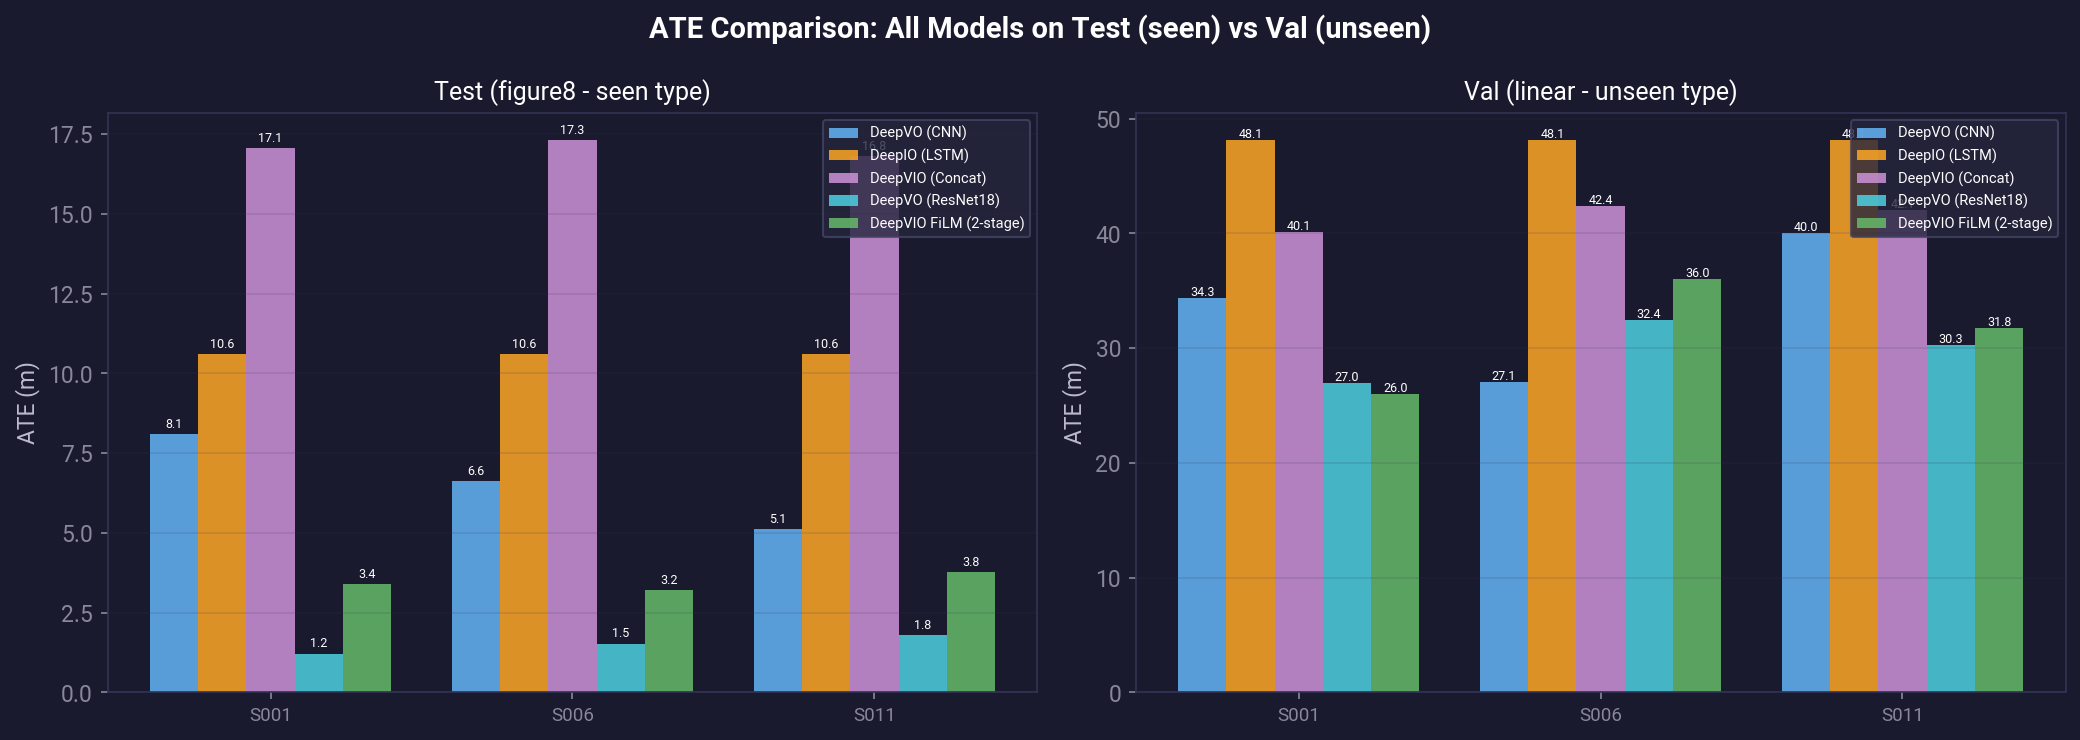
\includegraphics[width=\columnwidth]{visualizations/fig20_all_models_ate.png}
    \caption{ATE comparison across all models on test (seen trajectory type) vs validation (unseen linear trajectory). DeepIO degrades most on unseen trajectories (48.1m), while fusion models show more robust generalization.}
    \label{fig:ate_all}
\end{figure}

% ======================================================================
\section{Discussion}
% ======================================================================

\textbf{Data quality as the primary bottleneck.} Our most impactful finding is that data quality---not model architecture---was the primary bottleneck. Fixing textures and adding 3D scene geometry gave 40\% improvement before any model changes. This aligns with observations from TartanAir~\cite{wang2020tartanair} that diverse, feature-rich environments are essential.

\textbf{Pretrained features are essential.} The ResNet-18 encoder (11.4M params, ImageNet pretrained) achieved 90\% better test loss than a 4-layer CNN (735K params) trained from scratch. This confirms DeepVO's finding~\cite{wang2017} that pretrained visual features are critical for visual odometry.

\textbf{FiLM vs.\ concatenation.} FiLM conditioning provides a richer modality interaction than concatenation. By allowing the IMU to generate per-channel scale and shift for visual features, the model can learn to amplify motion-relevant visual channels and suppress noise, depending on the inertial context.

\textbf{Two-stage training.} The modality imbalance problem~\cite{wang2020multimodal} manifests clearly in our gate analysis. Without two-stage training, the IMU converges in 3 epochs and suppresses vision. Our solution---pretraining visual, freezing, then jointly finetuning---achieves balanced fusion ($\alpha \approx 0.47$) and the best overall performance.

\textbf{Limitations.} Our synthetic scenes use a single ground plane with primitives, far simpler than real environments. The dataset contains only 4 trajectory types and $\sim$12K training samples, orders of magnitude smaller than KITTI~\cite{geiger2012} or TartanAir~\cite{wang2020tartanair}. The single-pair prediction lacks temporal context that DeepVO's LSTM provides~\cite{wang2017}.

% ======================================================================
\section{Conclusion}
% ======================================================================

We presented a complete pipeline for deep visual-inertial odometry on synthetic data, from Blender-based data generation to FiLM-based sensor fusion. Our key contribution is demonstrating that the combination of (1) data quality curation, (2) pretrained visual features, (3) FiLM conditioning, and (4) two-stage training achieves a 92\% improvement over the baseline, with the fused model outperforming vision-only for the first time. The gate analysis provides interpretable evidence of balanced modality fusion.

Future work includes precomputed optical flow input~\cite{wang2021, teed2020}, temporal LSTM modeling over frame sequences, training on diverse 3D environments such as TartanAir~\cite{wang2020tartanair}, and evaluation on real-world VIO benchmarks such as EuRoC~\cite{burri2016}.

% ======================================================================
% REFERENCES
% ======================================================================
\begin{thebibliography}{15}

\bibitem{mourikis2007}
A.~I. Mourikis and S.~I. Roumeliotis, ``A Multi-State Constraint Kalman Filter for Vision-aided Inertial Navigation,'' in \textit{Proc. IEEE ICRA}, 2007, pp.~3565--3572.

\bibitem{qin2018}
T.~Qin, P.~Li, and S.~Shen, ``VINS-Mono: A Robust and Versatile Monocular Visual-Inertial State Estimator,'' \textit{IEEE Trans. Robotics}, vol.~34, no.~4, pp.~1004--1020, 2018.

\bibitem{wang2017}
S.~Wang, R.~Clark, H.~Wen, and N.~Trigoni, ``DeepVO: Towards End-to-End Visual Odometry with Deep Recurrent Convolutional Neural Networks,'' in \textit{Proc. IEEE ICRA}, 2017, pp.~2043--2050.

\bibitem{clark2017}
R.~Clark, S.~Wang, H.~Wen, A.~Markham, and N.~Trigoni, ``VINet: Visual-Inertial Odometry as a Sequence-to-Sequence Learning Problem,'' in \textit{Proc. AAAI}, 2017, pp.~3995--4001.

\bibitem{mur2015}
R.~Mur-Artal, J.~M.~M. Montiel, and J.~D. Tard\'{o}s, ``ORB-SLAM: A Versatile and Accurate Monocular SLAM System,'' \textit{IEEE Trans. Robotics}, vol.~31, no.~5, pp.~1147--1163, 2015.

\bibitem{wang2021}
W.~Wang, Y.~Hu, and S.~Scherer, ``TartanVO: A Generalizable Learning-based Visual Odometry,'' in \textit{Proc. CoRL}, 2021.

\bibitem{wang2020tartanair}
W.~Wang \textit{et al.}, ``TartanAir: A Dataset to Push the Limits of Visual SLAM,'' in \textit{Proc. IEEE/RSJ IROS}, 2020, pp.~4820--4827.

\bibitem{sun2018}
D.~Sun, X.~Yang, M.-Y. Liu, and J.~Kautz, ``PWC-Net: CNNs for Optical Flow Using Pyramid, Warping, and Cost Volume,'' in \textit{Proc. IEEE CVPR}, 2018, pp.~8934--8943.

\bibitem{han2019}
L.~Han, Y.~Lin, G.~Du, and S.~Lian, ``DeepVIO: Self-supervised Deep Learning of Monocular Visual-Inertial Odometry using 3D Geometric Constraints,'' in \textit{Proc. IEEE/RSJ IROS}, 2019, pp.~6906--6913.

\bibitem{chen2019}
C.~Chen \textit{et al.}, ``Selective Sensor Fusion for Neural Visual-Inertial Odometry,'' in \textit{Proc. IEEE CVPR}, 2019, pp.~10542--10551.

\bibitem{perez2018}
E.~Perez, F.~Strub, H.~de~Vries, V.~Dumoulin, and A.~Courville, ``FiLM: Visual Reasoning with a General Conditioning Layer,'' in \textit{Proc. AAAI}, 2018, pp.~3942--3951.

\bibitem{wang2020multimodal}
W.~Wang, D.~Tran, and M.~Feiszli, ``What Makes Training Multi-Modal Classification Networks Hard?'' in \textit{Proc. IEEE CVPR}, 2020, pp.~12695--12705.

\bibitem{burri2016}
M.~Burri \textit{et al.}, ``The EuRoC Micro Aerial Vehicle Datasets,'' \textit{Int. J. Robotics Research}, vol.~35, no.~10, pp.~1157--1163, 2016.

\bibitem{teed2020}
Z.~Teed and J.~Deng, ``RAFT: Recurrent All-Pairs Field Transforms for Optical Flow,'' in \textit{Proc. ECCV}, 2020, pp.~402--419.

\bibitem{he2016}
K.~He, X.~Zhang, S.~Ren, and J.~Sun, ``Deep Residual Learning for Image Recognition,'' in \textit{Proc. IEEE CVPR}, 2016, pp.~770--778.

\bibitem{dosovitskiy2015}
A.~Dosovitskiy \textit{et al.}, ``FlowNet: Learning Optical Flow with Convolutional Networks,'' in \textit{Proc. IEEE ICCV}, 2015, pp.~2758--2766.

\bibitem{geiger2012}
A.~Geiger, P.~Lenz, and R.~Urtasun, ``Are we ready for Autonomous Driving? The KITTI Vision Benchmark Suite,'' in \textit{Proc. IEEE CVPR}, 2012, pp.~3354--3361.

\bibitem{pech2000}
S.~Pertuz, D.~Puig, and M.~A. Garcia, ``Analysis of focus measure operators for shape-from-focus,'' \textit{Pattern Recognition}, vol.~46, no.~5, pp.~1415--1432, 2013.

\end{thebibliography}

\end{document}
